\chapter{Meranie réžie}
\label{ch:overhead}

Réžia sa meria podľa návrhu z časti~\ref{sec:measurement-design}: šesť konfigurácií sa strieda v piatich kolách, latencia sa meria pri konštantnej záťaži 2000 požiadaviek za sekundu medzi podmi fortio a 100 požiadaviek za sekundu cez aplikáciu, priepustnosť jedným tokom TCP. Tabuľky uvádzajú medián z piatich opakovaní a v zátvorke rozpätie od minima po maximum. Rozdiel sa pokladá za skutočný, iba ak sa rozpätia neprekrývajú. Všetky hodnoty pochádzajú z virtual machines na jednom notebooku, preto sú zmysluplné iba ich pomery (časť~\ref{sec:limits-validity}).

\section{Latencia}

Tabuľka~\ref{tab:latency} uvádza priemernú latenciu na troch cestách a percentily cesty cez aplikáciu. Priemer je presný; percentily ciest medzi podmi fortio sa počítajú z histogramu s krokom 10~\textmu s.

\begin{table}[ht!]
  \centering
  \caption{Latencia v ms pri konštantnej záťaži, medián [min--max] z piatich opakovaní}
  \label{tab:latency}
  \footnotesize
  \renewcommand{\arraystretch}{1.15}
  \begin{tabularx}{\textwidth}{@{}>{\raggedright\arraybackslash}X>{\centering\arraybackslash}p{2.0cm}>{\centering\arraybackslash}p{2.0cm}>{\centering\arraybackslash}p{2.0cm}>{\centering\arraybackslash}p{2.0cm}@{}}
    \toprule
    Konfigurácia & Jeden uzol, priemer & Medzi uzlami, priemer & Aplikácia, p50 & Aplikácia, p99 \\
    \midrule
    Bez ochrany & 0,150 & 0,515 & 15,6 & 23,1 \\
    Segmentácia siete & 0,156 & 0,507 & 15,9 & 23,9 \\
    Šifrovanie medzi uzlami & 0,154 & 0,578 & 17,3 & 24,9 \\
    Mesh bez mTLS & 0,651 & 0,912 & 16,5 & 24,3 \\
    mTLS medzi službami & 0,683 & 0,922 & 18,7 & 26,8 \\
    L7 autorizácia & 0,692 & 0,953 & 18,6 & 28,2 \\
    \bottomrule
  \end{tabularx}
\end{table}
% TODO: po opakovanom meraní latencie (beh 02.11) doplniť rozpätia a percentily p50/p99 ciest medzi podmi fortio; priemery overiť proti novému behu.

\begin{figure}[ht!]
  \centering
  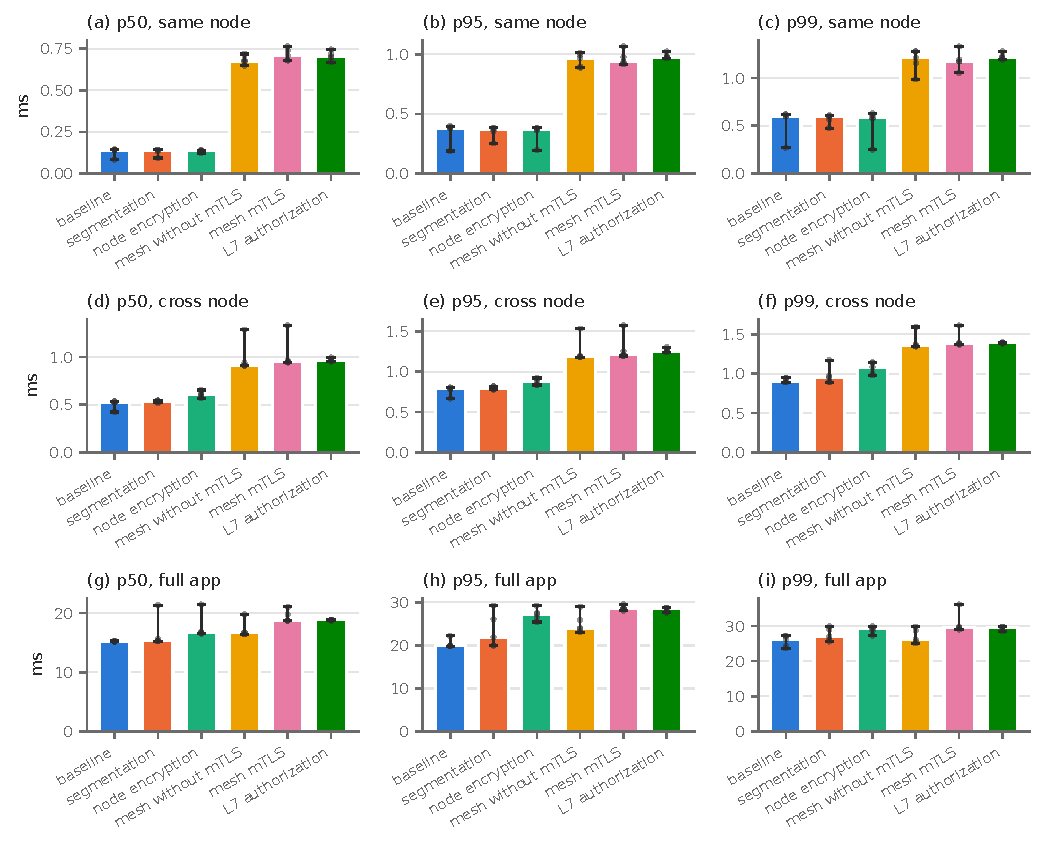
\includegraphics[width=\textwidth]{../figures/bench/latency.pdf}
  \caption{Latencia podľa konfigurácie a cesty}
  \label{fig:latency}
\end{figure}

\section{Priepustnosť a spotreba CPU}

Priepustnosť jedného toku TCP medzi uzlami je zhora obmedzená linkou medzi virtual machines: bez podov a CNI dosahuje 1,36~Gbit/s a pody v konfigurácii bez ochrany 1,34~Gbit/s (tabuľka~\ref{tab:throughput}). Rozdiely medzi konfiguráciami sa preto medzi uzlami prejavia hlavne ako spotreba CPU na prenesený gigabit. Na jednom uzle linka nebráni a priepustnosť priamo ukazuje cenu spracovania paketu.

\begin{table}[ht!]
  \centering
  \caption{Priepustnosť jedného toku TCP a spotreba CPU uzlov (milijadrá na Gbit/s bez nečinnej spotreby), medián [min--max]}
  \label{tab:throughput}
  \footnotesize
  \renewcommand{\arraystretch}{1.15}
  \begin{tabularx}{\textwidth}{@{}>{\raggedright\arraybackslash}X>{\centering\arraybackslash}p{2.2cm}>{\centering\arraybackslash}p{2.2cm}>{\centering\arraybackslash}p{2.0cm}>{\centering\arraybackslash}p{2.0cm}@{}}
    \toprule
    Konfigurácia & Jeden uzol, Gbit/s & Medzi uzlami, Gbit/s & CPU, jeden uzol & CPU, medzi uzlami \\
    \midrule
    Bez ochrany & 94,5 [92,2--94,7] & 1,34 [1,30--1,35] & 17 & 758 \\
    Segmentácia siete & 93,5 [89,3--93,9] & 1,33 [1,32--1,34] & 17 & 761 \\
    Šifrovanie medzi uzlami & 107 [106--108] & 1,17 [1,16--1,19] & 15 & 2020 \\
    Mesh bez mTLS & 58,4 [57,8--58,5] & 1,34 [1,33--1,35] & 45 & 1080 \\
    mTLS medzi službami & 25,7 [24,3--25,8] & 1,28 [1,27--1,30] & 88 & 1170 \\
    L7 autorizácia & 24,7 [24,4--26,2] & 1,27 [1,26--1,29] & 89 & 1180 \\
    \bottomrule
  \end{tabularx}
\end{table}

Šifrovanie medzi uzlami má na jednom uzle vyššiu priepustnosť než konfigurácia bez ochrany, hoci prevádzka na jednom uzle cez WireGuard vôbec neprechádza. Príčinou je menšie MTU: Cilium pri zapnutom WireGuard zníži MTU všetkých trás podov z 1450 na 1355~B, takže sa zmení aj veľkosť segmentu TCP (MSS 1303 namiesto 1398~B). Kontrolné meranie konfigurácie bez ochrany s rovnakým MTU a bez šifrovania dosiahlo 105,6 až 106,8~Gbit/s, zatiaľ čo v tom istom behu s pôvodným MTU 88,7 až 93,3~Gbit/s. Rozdiel teda spôsobuje MTU, nie šifrovanie. Rovnaké kontrolné meranie ukázalo medzi uzlami 1,2~Gbit/s, takže časť poklesu priepustnosti pri šifrovaní medzi uzlami pripadá tiež na menšie MTU.

\begin{figure}[ht!]
  \centering
  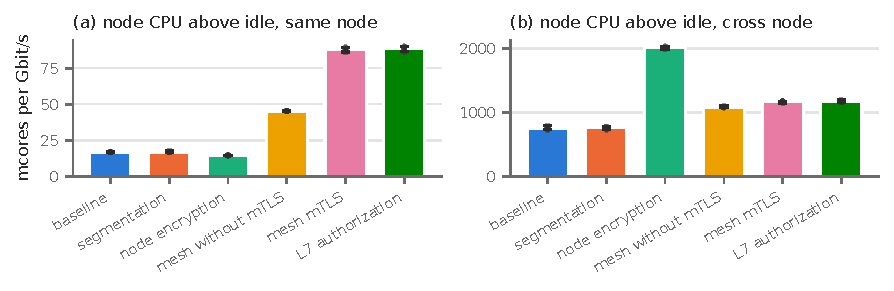
\includegraphics[width=\textwidth]{../figures/bench/cost-per-gbit.pdf}
  \caption{Spotreba CPU na prenesený Gbit/s podľa konfigurácie}
  \label{fig:cost-per-gbit}
\end{figure}

\section{Saturácia a pamäť}

Postupné zvyšovanie záťaže ukazuje, kde cesta prestane stíhať (obrázok~\ref{fig:qps-sweep}). Medzi uzlami zvládne konfigurácia bez ochrany najviac približne 26~500 požiadaviek za sekundu, šifrovanie medzi uzlami 20~900 a všetky konfigurácie s mesh okolo 10~500. Cez aplikáciu klesne maximum z 462 na 367 až 378 požiadaviek za sekundu. Pevné záťaže z tabuľky~\ref{tab:latency} ležia pod 30~\% najnižšieho z týchto maxím, takže latencia nie je meraná pri saturácii.

\begin{figure}[ht!]
  \centering
  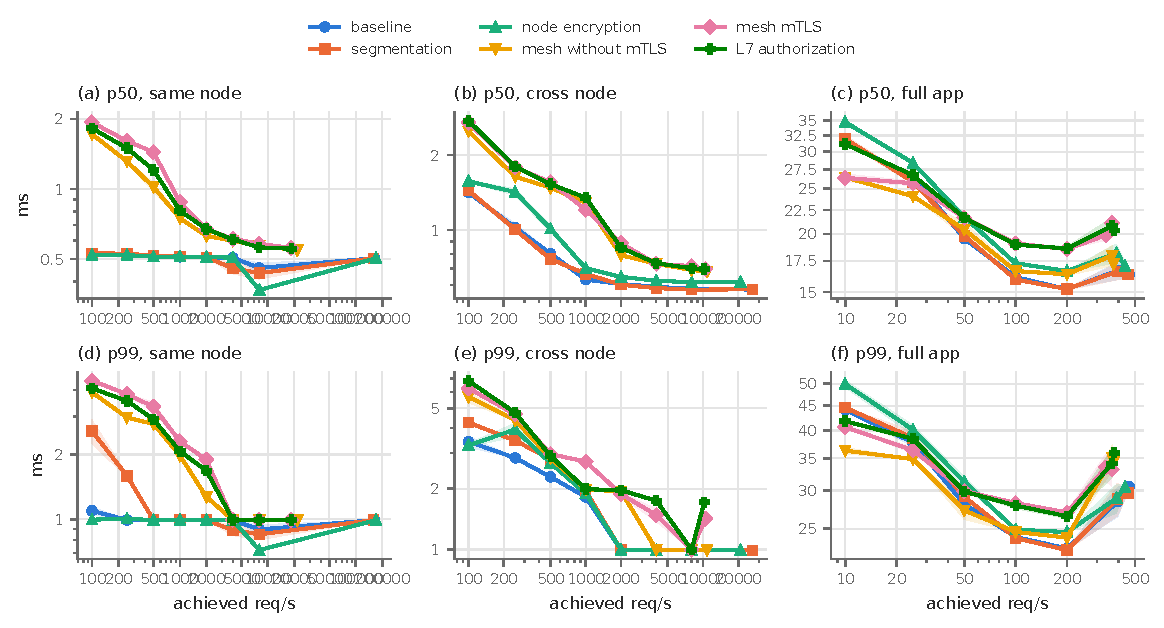
\includegraphics[width=\textwidth]{../figures/bench/qps-sweep.pdf}
  \caption{Latencia pri rastúcej záťaži}
  \label{fig:qps-sweep}
\end{figure}

Mesh zvýši pamäť každého uzla približne o 200~MiB: sidecar zaberá okolo 29~MiB na pod a riadiaca rovina istiod 46~MiB. Šifrovanie medzi uzlami a segmentácia siete pamäť merateľne nemenia.

\section{Réžia jednotlivých prvkov}
\label{sec:deltas}

Tabuľka~\ref{tab:deltas-measured} priraďuje namerané rozdiely porovnávaným dvojiciam z tabuľky~\ref{tab:deltas}.

\begin{table}[ht!]
  \centering
  \caption{Réžia jednotlivých prvkov}
  \label{tab:deltas-measured}
  \footnotesize
  \renewcommand{\arraystretch}{1.15}
  \begin{tabularx}{\textwidth}{@{}>{\raggedright\arraybackslash}p{3.6cm}>{\raggedright\arraybackslash}X@{}}
    \toprule
    Prvok & Nameraný rozdiel \\
    \midrule
    NetworkPolicy v eBPF & v rámci rozptylu vo všetkých veličinách \\
    WireGuard medzi uzlami & medzi uzlami +0,07~ms (+14~\%), aplikácia +1,4~ms (p50); priepustnosť $-$12~\%, CPU na Gbit/s 2,7-krát vyššie; na jednom uzle bez vplyvu \\
    Sidecar proxy bez šifrovania & +0,5~ms na jednom uzle (4,2-krát), +0,4~ms medzi uzlami, aplikácia +0,6~ms; priepustnosť na jednom uzle $-$38~\%; maximum medzi uzlami z 26~400 na 10~800 požiadaviek/s; +200~MiB pamäte na uzol \\
    mTLS v proxy & na ceste medzi podmi +0,01 až 0,03~ms, aplikácia +2,2~ms (+13~\%); priepustnosť na jednom uzle $-$56~\%, CPU na Gbit/s na jednom uzle 2,0-krát vyššie \\
    mTLS oproti WireGuard & mTLS má o 0,34~ms vyššiu latenciu medzi uzlami a o 1,4~ms cez aplikáciu, ale medzi uzlami spotrebuje o 42~\% menej CPU na Gbit/s a má vyššiu priepustnosť \\
    L7 autorizácia & medzi uzlami +0,03~ms (+3~\%), na hranici rozptylu; ostatné veličiny v rámci rozptylu \\
    \bottomrule
  \end{tabularx}
\end{table}

Väčšinu ceny mesh tvorí samotný sidecar, nie šifrovanie: každá požiadavka prejde dvakrát cez proxy v používateľskom priestore. mTLS pridá na krátkej ceste medzi podmi málo, no cez aplikáciu so štyrmi skokmi pridá viac než samotné sidecary. WireGuard je pri latencii lacnejší, lebo šifruje v jadre bez prechodu do používateľského priestoru, ale pri objemovom prenose medzi uzlami spotrebuje na gigabit viac CPU než mTLS. Segmentácia siete a L7 autorizácia sú pri tejto záťaži prakticky zadarmo.
